%%%%%%%%%%%%%%%%%%%%%%%%%%%%%%%%%%%%%%%%%%%%%%%%%%%%%%%%%%%%%%%%%%%%%%%%%%%%%%%%
%2345678901234567890123456789012345678901234567890123456789012345678901234567890
%        1         2         3         4         5         6         7         8

\documentclass[letterpaper, 10 pt, conference]{ieeeconf}  % Comment this line out if you need a4paper

%\documentclass[a4paper, 10pt, conference]{ieeeconf}      % Use this line for a4 paper

\IEEEoverridecommandlockouts                              % This command is only needed if 
                                                          % you want to use the \thanks command

\overrideIEEEmargins                                      % Needed to meet printer requirements.

%In case you encounter the following error:
%Error 1010 The PDF file may be corrupt (unable to open PDF file) OR
%Error 1000 An error occurred while parsing a contents stream. Unable to analyze the PDF file.
%This is a known problem with pdfLaTeX conversion filter. The file cannot be opened with acrobat reader
%Please use one of the alternatives below to circumvent this error by uncommenting one or the other
%\pdfobjcompresslevel=0
%\pdfminorversion=4

% See the \addtolength command later in the file to balance the column lengths
% on the last page of the document

% The following packages can be found on http:\\www.ctan.org
\usepackage{graphics} % for pdf, bitmapped graphics files
\usepackage{xcolor} % for coloring
\usepackage{epsfig} % for postscript graphics files
\usepackage{booktabs} % for tables
\usepackage{multirow} % for tables
\usepackage{mathptmx} % for math equations
\usepackage{amsmath} % for math equations
\usepackage{amssymb}
\usepackage{float}
\usepackage{hyperref}
\hypersetup{
    colorlinks=true,
    urlcolor=blue
}
\usepackage{tikz}
\usetikzlibrary{arrows.meta, positioning, calc}
\usepackage{caption}
\captionsetup[table]{name=Table, labelsep=colon}
\definecolor{mybluebg}{RGB}{198,228,252}


% \title{\LARGE \bf
% Evaluating the Effectiveness of Haptic Force Feedback during Data Collection for Force-Aware Visuomotor Policy Learning
% }
\title{\LARGE \bf
Modeling Kinematic Signatures of Aging for Human Motion Prediction in Assistive Robotics
%Age-Conditioned Human Motion Generation for Assistive Robot Anticipation
}


% If anonymized:
%\author{Anonymous Author(s)}

% If non-anonymized, use the standard author block:
% \author{First Author\\Institution\\{\tt\small email} \and Second Author\\Institution\\{\tt\small email}}
\author{
Yiran Liu$^{1,2}$, Eugene Zhao$^{1,2}$, Karim Habashy$^{1,2}$, Jason Peng$^{3}$, Chang Shu$^{1}$, Pengcheng Xi$^{1}$ \\
$^{1}$National Research Council Canada \quad
$^{2}$University of Waterloo \quad
$^{3}$Simon Fraser University \\
{\tt\small y3275liu@uwaterloo.ca, chang.shu@nrc-cnrc.gc.ca, pengcheng.xi@nrc-cnrc.gc.ca}
}


\begin{document}



\maketitle
% \thispagestyle{empty}
% \pagestyle{empty}

%%%%%%%%%%%%%%%%%%%%%%%%%%%%%%%%%%%%%%%%%%%%%%%%%%%%%%%%%%%%%%%%%%%%%%%%%%%%%%%%
\begin{abstract}
We present an age-conditioned human motion generation framework for studying aging signatures in the context of assistive robotics.
Our pipeline converts clinical gait recordings into learning-ready motion representations while addressing defects from legacy motion-capture data.
Using 420 clips from 138 subjects across young, mid-age, and elderly groups, we train a Spatial-Temporal Graph Convolutional Network (ST-GCN) to recognize age group from motion clips, achieving 64.6\% classification accuracy.
We then fine-tune a Motion Diffusion Model (MDM) with Low-Rank Adaptation (LoRA) to generate text-conditioned human motion with age-group control, and compare against the unadapted MDM under both neutral and elderly-described text prompts.
To evaluate whether generated motions preserve aging-related characteristics, we analyze clinical and kinematic gait metrics on 9{,}000 generated clips.
Our results show that the LoRA-adapted model reproduces spatial kinematic constraints in the Elderly condition --- a signature the unadapted MDM fails to express even under elderly-described prompts --- but spatiotemporal consistency remains unresolved, with generated stride variability massively overshooting clinical baselines, which we attribute to the capacity ceiling of low-rank, discrete-token adaptation.
These findings highlight dataset size, motion quality, and conditioning strength as key bottlenecks, and motivate larger age-diverse datasets for demographic-aware motion prediction and assistive robot planning.
Code and video available on the \href{https://catr1xliu.github.io/Notebook/Aging-Motion-Project/}{project page}.
\end{abstract}

%%%%%%%%%%%%%%%%%%%%%%%%%%%%%%%%%%%%%%%%%%%%%%%%%%%%%%%%%%%%%%%%%%%%%%%%%%%%%%%%
\section{INTRODUCTION}

\begin{figure*}[t]
	\centering
	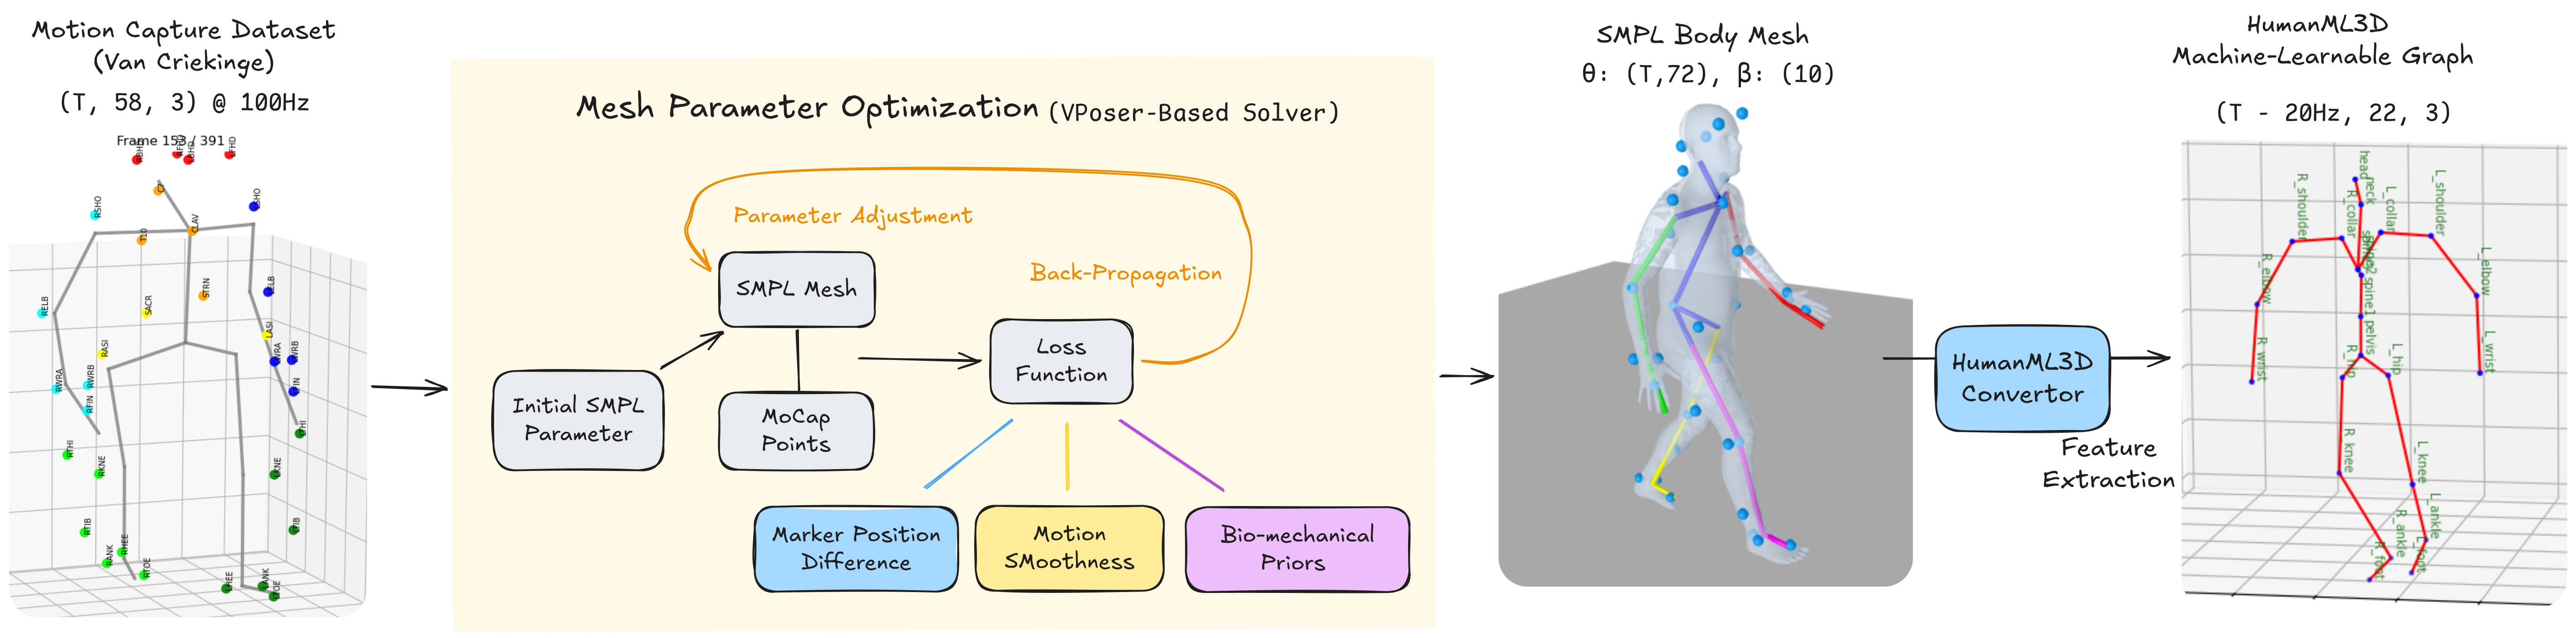
\includegraphics[width=0.7\textwidth]{sec/figs/18 - Data Pipeline Diagram.png}

	\vspace{0.6em}

	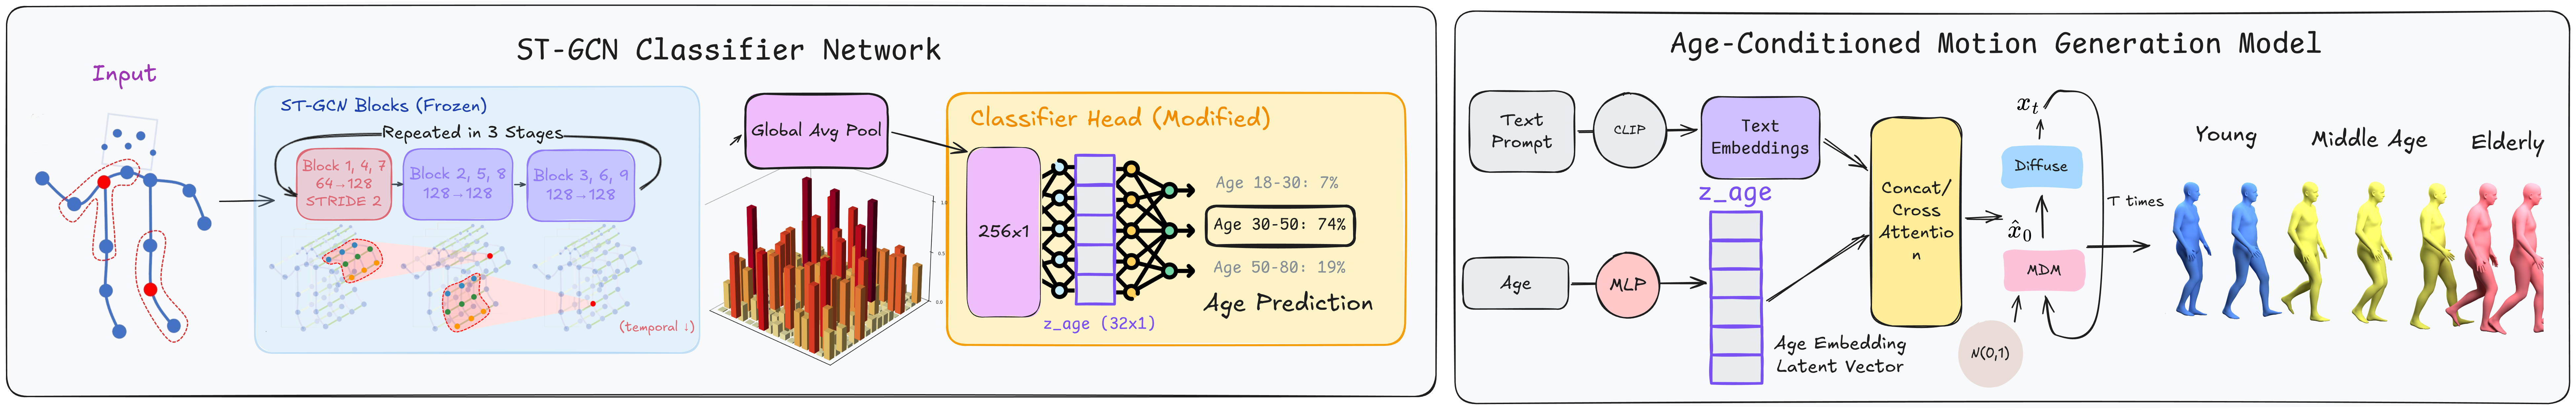
\includegraphics[width=\textwidth]{sec/figs/24 - Revised Motion Generation Model.png}
	\caption{Overview of our age-aware motion synthesis framework. \emph{Top:} clinical marker recordings are converted into the 263-dimensional HumanML3D representation via VPoser-regularized SMPL fitting followed by feature extraction. \emph{Bottom:} an ST-GCN++ age representation learner extracts $\mathbf{z}_\text{age}$ (left) and an age-conditioned Motion Diffusion Model (right) generates text-driven motion.}
	\label{fig:framework}
\end{figure*}

Accurate human motion anticipation is foundational for safe human-robot interaction, especially when robots share space with humans, plan around future movement, or provide proactive assistance.
Recent deep generative architectures, particularly Motion Diffusion Models (MDMs)~\cite{tevet2023human, chen2022mld}, have demonstrated strong capability in synthesizing realistic and diverse human motions.
However, widely used motion-capture datasets such as AMASS~\cite{mahmood2019amass} are heavily biased toward young, healthy actors~\cite{umagami2025intend}, so existing generative models cover diverse actions and styles~\cite{sawdayee2025dance} but rarely capture population-level biomechanical factors such as age~\cite{liao2025shapemovestextdrivenshapeaware}.
This limitation is particularly critical for assistive robots in aging-in-place and eldercare scenarios, where anticipating older adults' movements is essential for safe navigation, timely assistance, and proactive interaction.

Although MDMs are trained for synthesis rather than direct forecasting, they implicitly learn the distribution over plausible future motions --- precisely what a prediction system samples from under partial observation.
Age-conditioning this distribution restricts samples to a demographic-specific manifold, giving downstream forecasters and robot planners priors aligned to the user population they serve.
An age-aware generative prior is therefore a precursor to, rather than a substitute for, motion prediction in eldercare contexts; clinical gait analysis, which has long quantified spatiotemporal aging signatures~\cite{diaz2025evaluating, galasso2024development}, provides the supervision signal needed to build it.

To address this gap, we present a proof-of-concept framework that integrates clinical gait analysis with deep generative modeling toward age-aware human motion synthesis.
We develop a data processing pipeline that converts clinical gait recordings into standardized skeletal representations, fine-tune a Spatial-Temporal Graph Convolutional Network (ST-GCN)~\cite{yan2018stgcn} to infer age group and encode age-related biomechanical characteristics into a latent representation, and train a Low-Rank Adaptation (LoRA)~\cite{hu2022lora} adapter for an MDM to generate text-driven motions conditioned on age group.
We evaluate generated motions with clinical and kinematic gait metrics and against the unadapted MDM under both neutral and elderly-described prompts.
Our analysis shows that the adapted model captures spatial kinematic constraints (reduced hip Range-of-Motion in the Elderly condition) that the unadapted MDM fails to express even when prompted explicitly for old age, but fails to reproduce spatiotemporal consistency: stride variability overshoots clinical baselines, a limitation we attribute to the capacity ceiling of low-rank, discrete-token adaptation.
These findings motivate larger, age-diverse human motion datasets and stronger conditioning mechanisms for downstream motion prediction and assistive robot planning.


%%%%%%%%%%%%%%%%%%%%%%%%%%%%%%%%%%%%%%%%%%%%%%%%%%%%%%%%%%%%%%%%%%%%%%%%%%%%%%%%
\section{METHODOLOGY: AGE-AWARE MOTION SYNTHESIS FRAMEWORK}
\label{sec:method}
\subsection{Data Processing Pipeline}
We adopt the motion capture dataset of Van Criekinge et al.~\cite{vancriekinge2023dataset} (ages 21--86) and convert clinical marker recordings into HumanML3D-format skeletal graphs~\cite{guo2022generating} via SMPL body-model fitting~\cite{mahmood2019amass} and feature extraction, as summarized in Fig.~\ref{fig:framework} (top).
As shown in Fig.~\ref{fig:artifact}, naive mapping causes mesh inflation (right), while standard priors induce crouch artifacts (left); our multi-stage optimization pipeline adapted from VPoser~\cite{pavlakos2019expressivebodycapture3d} addresses both to recover a natural posture (center) and resolves common clinical-dataset defects such as axis misalignment, marker mislabeling, and foot contact issues.

\begin{figure}[H]
	\centering
	\IfFileExists{sec/figs/BodyArtifacts.png}%
	{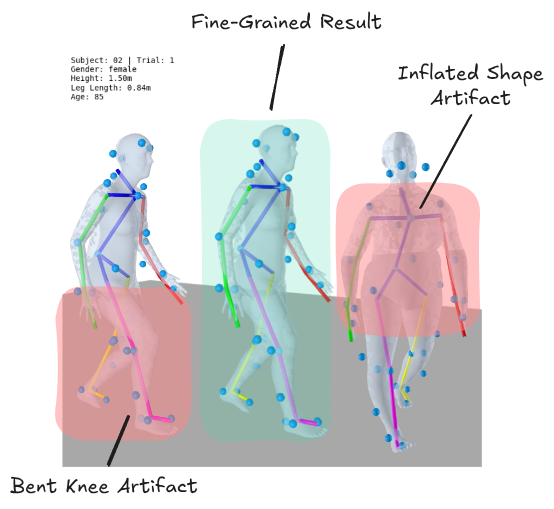
\includegraphics[width=0.7\linewidth]{sec/figs/BodyArtifacts.png}}%
	{\fbox{\parbox[c][4cm][c]{\linewidth}{\centering Artifact image missing: \texttt{sec/figs/BodyArtifacts.png}}}}
	\caption{Artifact analysis in clinical motion retargeting.}
	\label{fig:artifact}
\end{figure}

\subsection{Age Signature Detecting Network}
As illustrated in Fig.~\ref{fig:framework} (bottom left), an Age Representation Learner built on an ST-GCN~\cite{yan2018stgcn} is fine-tuned to classify motion clips into three age groups (Young, Mid, Elderly) and regress biological age.
Once the network can successfully predict age, the penultimate layer encapsulates the biomechanical signatures of aging (e.g., joint motion range).
We extract this vector to serve as the age latent embedding, denoted as $\mathbf{z}_{age}$.

\subsection{Age-Conditioned Generative Network}
Our target framework, shown in Fig.~\ref{fig:framework} (bottom right), is a Conditional Diffusion Model~\cite{tevet2023human, chen2022mld} that denoises a latent motion representation $\mathbf{x}_T$ conditioned on both text and age.
At training time, $\mathbf{z}_\text{age}$ extracted by the frozen ST-GCN encoder is injected via cross-attention, while a small MLP $g(a)$ is jointly trained to map a scalar age to the same latent space, enabling continuous age-controlled generation at inference from a desired age value alone.

Training this full architecture from scratch is infeasible under our compute and dataset budget, so the experiments in this paper validate a discrete-token prototype instead: we apply Low-Rank Adaptation (LoRA)~\cite{hu2022lora} to a pre-trained MDM with three style tokens (\texttt{young}, \texttt{mid}, \texttt{old}) and treat the continuous-conditioning architecture as the natural next step rather than a delivered contribution.
This honest scoping isolates the bottlenecks that future continuous conditioning must overcome.

\subsection{Gait-Analysis Metrics for Evaluation}
In order to validate that the aging signal is preserved in the processed dataset and successfully reproduced in the generated motion clips, we adapted several standard, training-free gait-analysis metrics documented in clinical literature~\cite{bailey2023smartwatch, cordeiro2025constraint, galasso2024development}.
\begin{itemize}
    \item \textbf{Spatiotemporal Parameters:} We compute average walking speed, stride length, and cadence by detecting heel-strike events based on the zero-velocity crossings of the ankle joints. 
    \item \textbf{Gait Variability:} We calculate the Coefficient of Variation (CV) for stride length and stride time across multiple steps. 
    \item \textbf{Joint Range of Motion (RoM):} We measure the peak flexion and extension angles of the hip and knee joints during the gait cycle. 
\end{itemize}
These metrics are computed deterministically from sample clips within our dataset and from motion generated by our LoRA-based prototype, providing a quantitative, biomechanically grounded evaluation of our framework.


%%%%%%%%%%%%%%%%%%%%%%%%%%%%%%%%%%%%%%%%%%%%%%%%%%%%%%%%%%%%%%%%%%%%%%%%%%%%%%%%
%\clearpage
\section{EXPERIMENTS AND RESULTS}

\subsection{Data Quality Validation}
The Van Criekinge et al.~\cite{vancriekinge2023dataset} clinical motion capture dataset contains recordings from 138 subjects across the lifespan.
During preprocessing, we resolved dataset-specific artifacts including sensor measurement errors, initialization transients, and mislabeled markers; after discarding 138 T-pose calibration clips, 24 short clips ($<40$ frames), and 4 manually identified artifact clips, the data loader yields 420 effective walking clips (Young 115 / Mid-age 154 / Elderly 151).
To preserve biological fidelity during conversion to the HumanML3D machine-learnable format, we applied a multi-stage optimization procedure adapted from VPoser~\cite{pavlakos2019expressivebodycapture3d}: the optimizer first recovers global body pose, then refines localized artifacts around body shape and limbs.
The fitting loss converges rapidly and eliminates the mesh-inflation and crouch-walking artifacts of Fig.~\ref{fig:artifact}; the converged residual is non-zero, reflecting legacy marker layout and remaining occlusion errors that contribute to the within-group variance visible in our distributional comparisons.

\subsection{Model Training Results}

\subsubsection{ST-GCN Age Representation Learner}
We fine-tuned the ST-GCN++ architecture to classify the processed walking clips into three age categories: Young ($<35$), Mid-age (35--60), and Elderly ($\geq60$).

\begin{figure}[H]
	\centering
	\begin{minipage}[t]{0.49\linewidth}
		\centering
		\IfFileExists{sec/figs/stgcn_train_loss.png}%
		{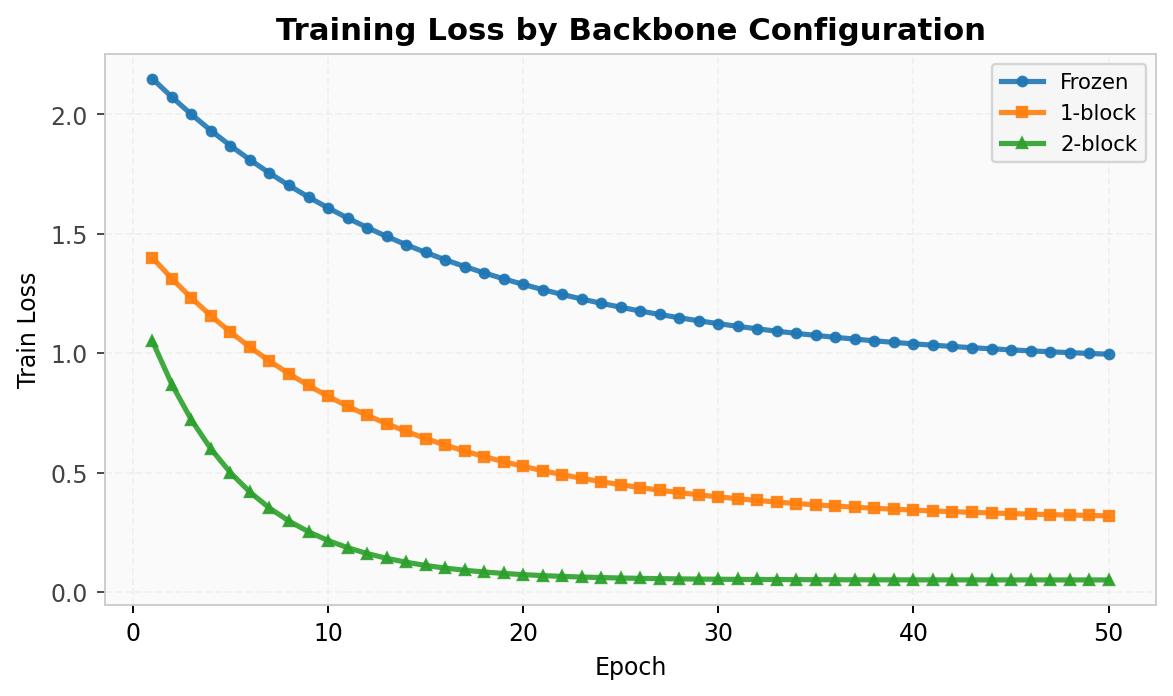
\includegraphics[width=\linewidth]{sec/figs/stgcn_train_loss.png}}%
		{}
	\end{minipage}\hfill
	\begin{minipage}[t]{0.49\linewidth}
		\centering
		\IfFileExists{sec/figs/stgcn_val_accuracy.png}%
		{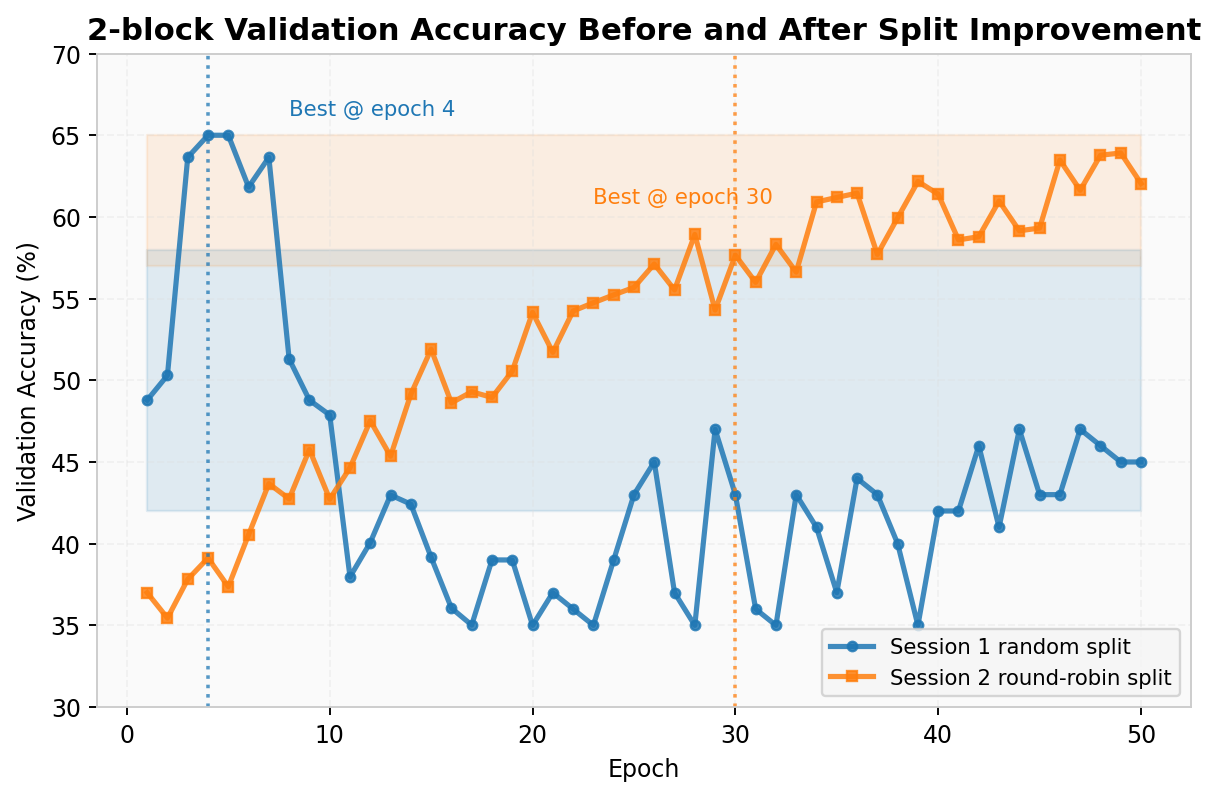
\includegraphics[width=\linewidth]{sec/figs/stgcn_val_accuracy.png}}%
		{}
	\end{minipage}
	\caption{Training dynamics for the ST-GCN age classifier. Left: training loss. Right: validation accuracy.}
	\label{fig:stgcn_curves}
\end{figure}

\begin{figure}[H]
	\centering
	\IfFileExists{sec/figs/stgcn_confusion.png}%
	{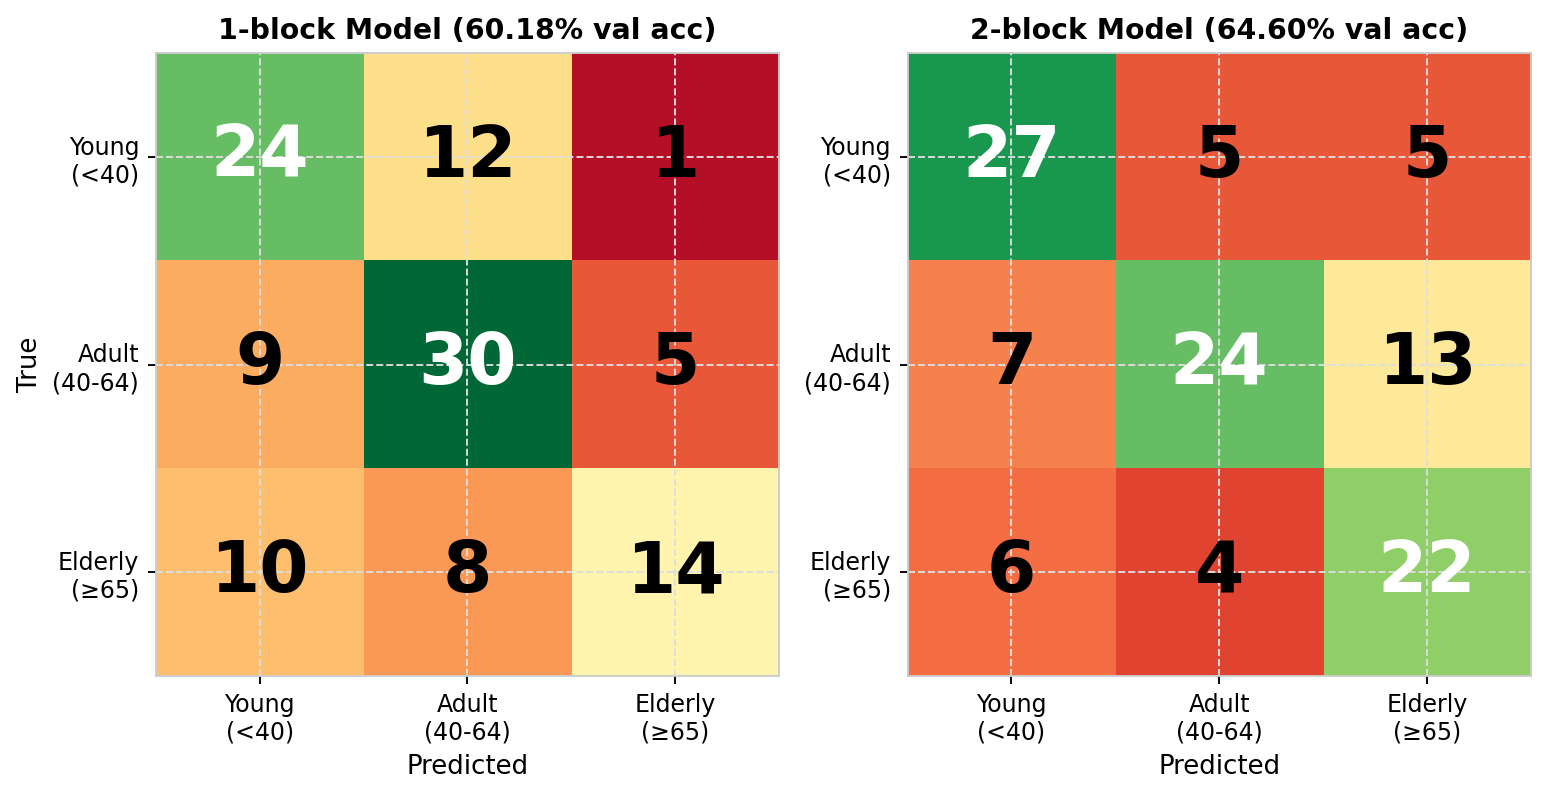
\includegraphics[width=0.8\linewidth]{sec/figs/stgcn_confusion.png}}%
	{}
	\caption{Confusion matrices for the ST-GCN predictions.}
	\label{fig:stgcn_confusion}
\end{figure}

These boundaries are not arbitrary: they roughly balance clip counts across bins and align with clinical findings that the kinematic gap between Young and Mid-age is small relative to within-group variance, whereas distinguishable spatiotemporal decline becomes consistent past 60~\cite{herssens2020investigation}.
To prevent subject-based overfitting --- where the model memorizes individual gait patterns --- we ensured strict, mutually exclusive subject assignment between training and validation, with an approximate 3:1 clip split (315 train / 105 validation clips, subject-disjoint across the 138 subjects).
We progressively unfreeze backbone blocks (Fig.~\ref{fig:stgcn_curves}) to balance validation accuracy (64.60\%) against overfitting, which remains visible as a gap between validation accuracy and the near-perfect training fit.
The confusion matrices (Fig.~\ref{fig:stgcn_confusion}) show that the model consistently separates the kinematic extremes (Young vs. Elderly), with the primary failure mode being the fragmentation of the Mid-age category --- a feature, not only a bug, given the small Young$\leftrightarrow$Mid kinematic gap reported in clinical studies.
We therefore report quantitative trends as Young$\to$Elderly contrasts and include Mid-age as a smooth interior point rather than a hard binary boundary.

\begin{figure*}[!t]
	\centering
	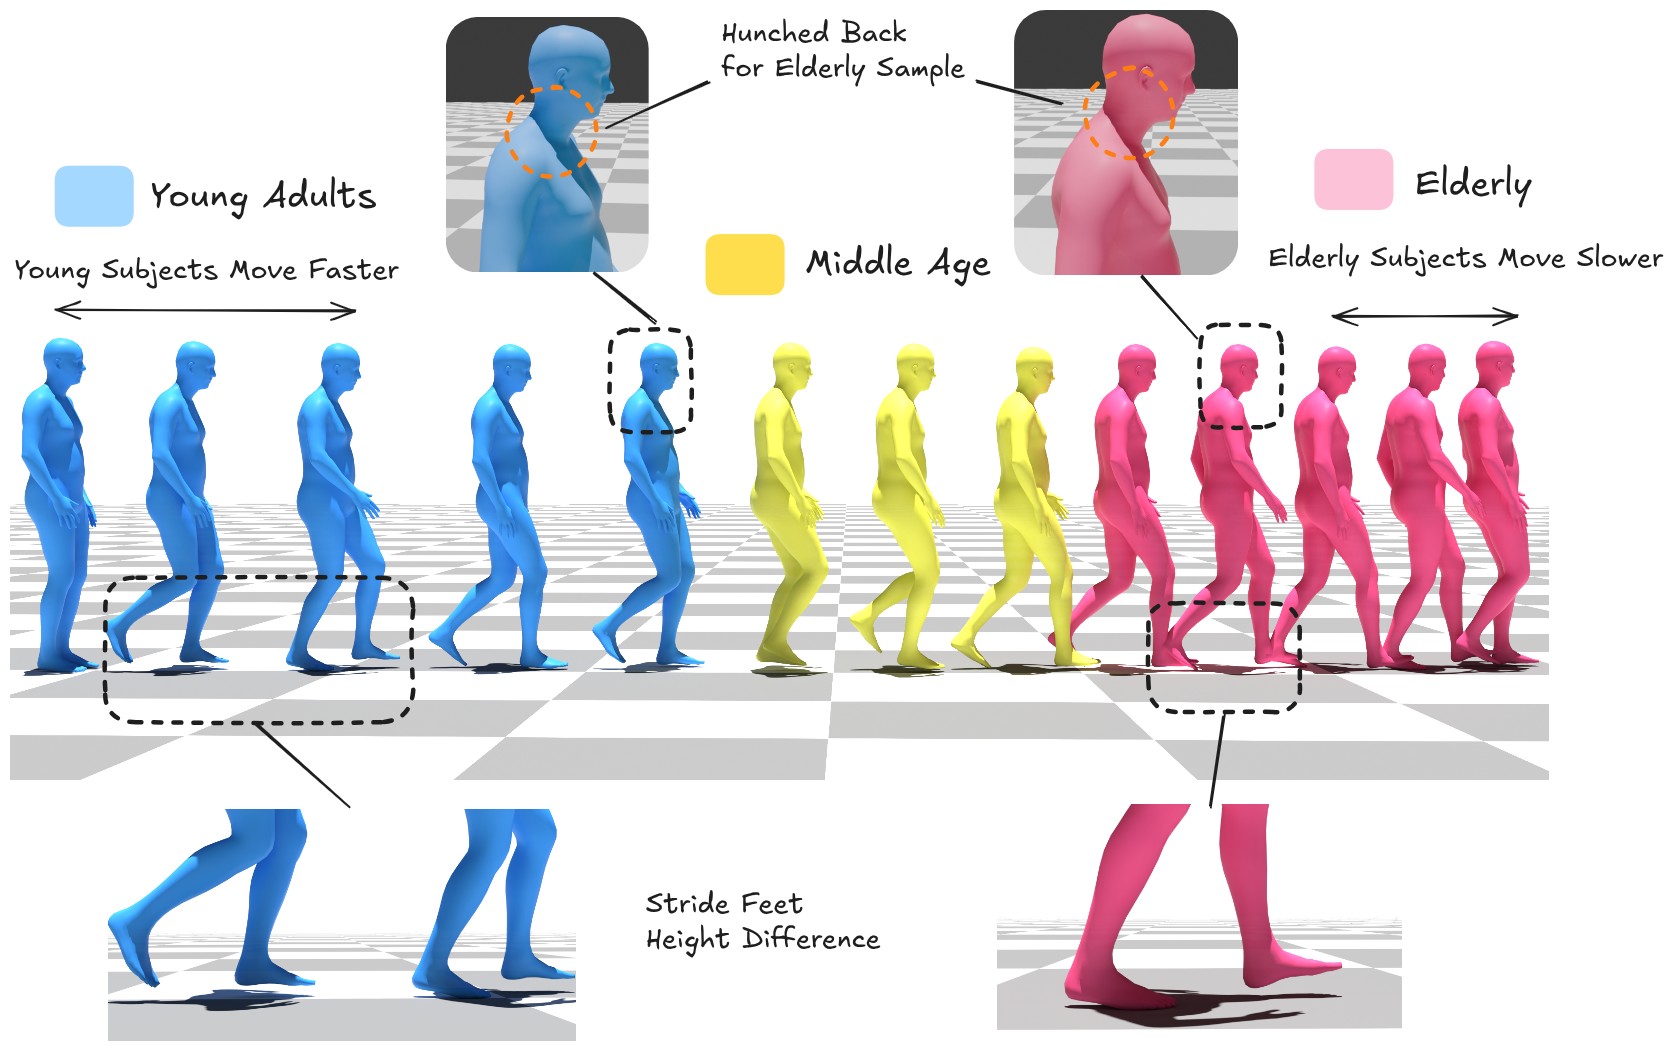
\includegraphics[width=0.7\textwidth]{sec/figs/25 - Generation Result.png}
	\caption{Generated walking sequences across the three age tokens (\texttt{young}, \texttt{mid}, \texttt{old}). The Elderly sample shows a noticeably hunched back and reduced foot-clearance height relative to the Young sample.}
	\label{fig:qualitative}
\end{figure*}
\subsubsection{Generative Motion Synthesis}
As a proof of concept, we conditioned the LoRA-adapted MDM using discrete age tokens.
After training LoRA adapters at ranks 5, 12, and 16, we selected the lowest-loss adapter (rank 12) and generated 3{,}000 clips per age condition (9{,}000 total) from the styled prompt template
\textit{``A person is walking forward in \{\textnormal{young}/\textnormal{mid}/\textnormal{old}\} style''}, with classifier-free guidance scale $s = 1.0$ to remain within the conditional distribution learned during LoRA training.
To isolate the effect of the adapter, we additionally generated baseline clips from the \textit{unadapted} MDM using a neutral prompt \textit{``A person is walking forward.''} and an explicit-age prompt \textit{``An old person is walking forward.''}.

\subsection{Quantitative Clinical Analysis}
We computed standard clinical metrics (Spatiotemporal Parameters, Gait Variability, and Joint Range of Motion) on both the processed ground-truth dataset and the 9,000 generated motion clips.

\subsubsection{Dataset Baseline Validation}
Analysis of the ground-truth dataset confirms that the expected aging signal is preserved end-to-end through our conversion pipeline: monotonic Young$\to$Elderly trends consistent with clinical literature are visible for walking speed, stride length, knee RoM, and stride-time CV (Fig.~\ref{fig:clinical_eval}), and per-clip linear regressions against chronological age (Fig.~\ref{fig:age_regression}) reproduce these directions with weak-to-moderate correlations.

\begin{figure}[H]
	\centering
	\IfFileExists{sec/figs/dataset/age_regression.png}%
	{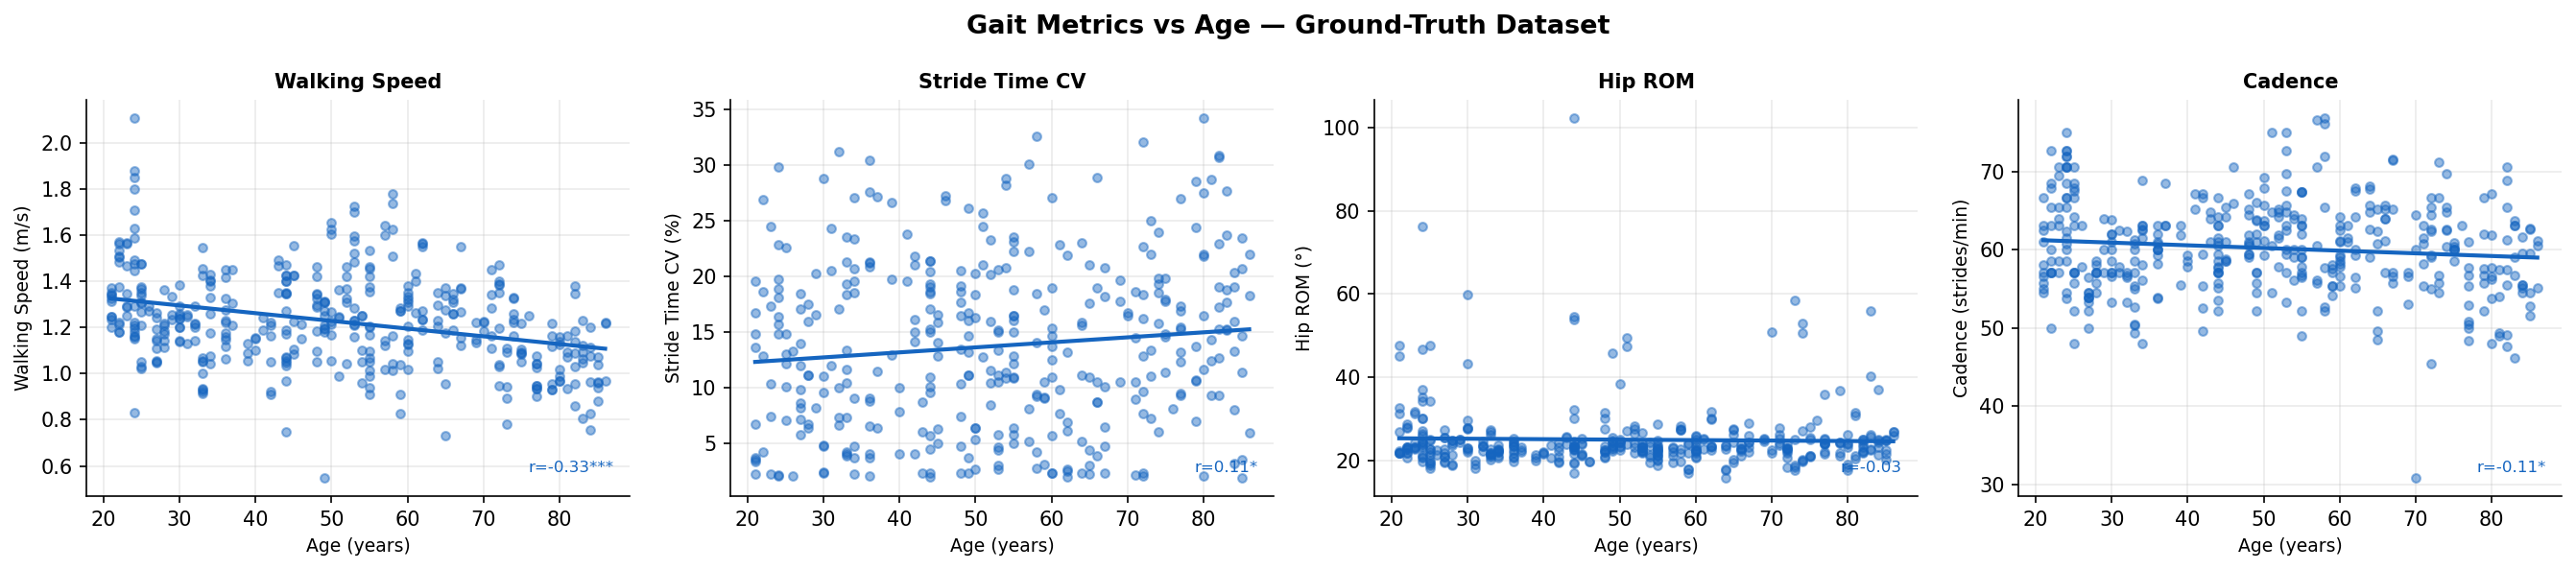
\includegraphics[width=\linewidth]{sec/figs/dataset/age_regression.png}}%
	{}
	\caption{Per-clip linear regression of clinical gait metrics against chronological age on the processed VC dataset.}
	\label{fig:age_regression}
\end{figure}

\subsubsection{Generated Result}
Fig.~\ref{fig:qualitative} shows representative motion sequences generated from the LoRA-adapted MDM under each age token. Coarse stylistic cues of aging are visible: the Elderly sample exhibits a noticeably hunched back, and stride-to-stride foot-clearance height differs visibly between the Young and Elderly conditions. Visual inspection alone is, however, an unreliable proxy for the underlying biomechanics, motivating the quantitative analysis below.

\subsubsection{Quantitative Gait Metrics Comparison}

\begin{figure}[H]
	\centering
	\IfFileExists{sec/figs/combined/combined_violin.png}%
	{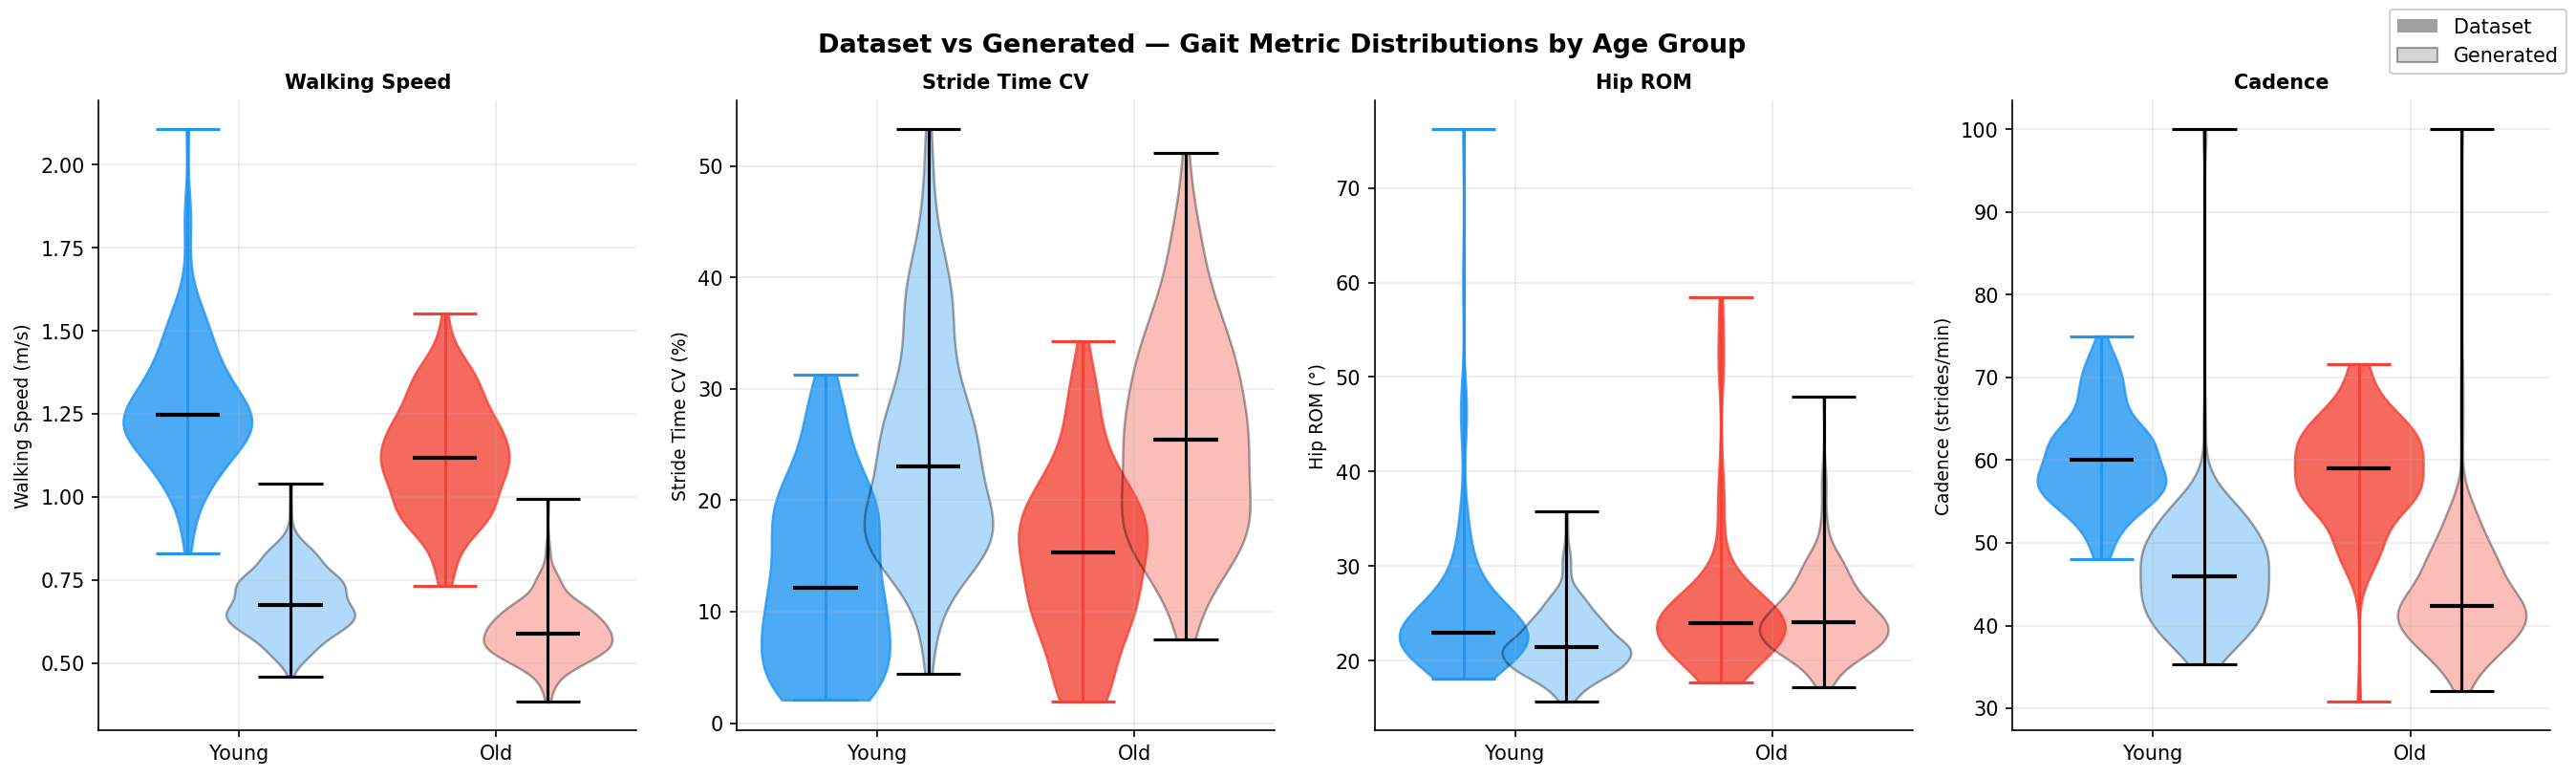
\includegraphics[width=\linewidth]{sec/figs/combined/combined_violin.png}}%
	{\fbox{\parbox[c][2cm][c]{\linewidth}{\centering Plot missing: \texttt{sec/figs/combined/combined\_violin.png}}}}
	\caption{Violin plots comparing the distribution of clinical metrics between the ground-truth dataset and the generated motion clips across age groups.}
	\label{fig:clinical_eval}
\end{figure}

\begin{table}[H]
\centering
\footnotesize
\caption{Welch two-sided $t$-test of Young$-$Old contrast on per-clip metrics at confidence level $\mathbf{C=95\%}$. Values in \textcolor{red}{red} are not statistically significant ($p\!\geq\!0.05$).}
\label{tab:welch}
\setlength{\tabcolsep}{6pt}
\begin{tabular}{lcc}
\toprule
\textbf{Metric (Y$-$O)} & \textbf{Dataset} $\Delta$ & \textbf{Generated} $\Delta$ \\
\midrule
Walking Speed (m/s)     & $+0.155$ & $+0.047$ \\
Stride-Time CV (\%)     & \textcolor{red}{$-1.87$} & \textcolor{red}{$-0.20$} \\
Hip RoM ($^\circ$)      & \textcolor{red}{$-0.25$} & $-0.65$ \\
Cadence (steps/min)     & $+1.61$ & $+1.64$ \\
Joint Lin.\ Vel.\ (m/s) & $+0.140$ & $+0.046$ \\
\bottomrule
\end{tabular}
\end{table}

Table~\ref{tab:welch} reports Welch two-sided $t$-tests of the Young$-$Old contrast on per-clip metrics, on both the dataset and the 9{,}000 LoRA-generated clips. Generated motions reproduce the expected sign and significance for walking speed, cadence, and joint linear velocity; hip RoM becomes significant only in the generated condition ($p\!=\!0.019$), so the adapter sharpens spatial constraints rather than merely mirroring them --- an effect the unadapted-MDM baselines (which fall within the \texttt{young}-token RoM range under both neutral and elderly-described prompts) cannot produce from text alone, confirming that the AMASS prior concentrates on young, healthy actors. Stride-time CV, however, remains non-significant and uniformly elevated (16--19\%) across all generated clips, far exceeding clinical reference values --- a failure we attribute in the Discussion to the capacity ceiling of low-rank, discrete-token adaptation rather than to text conditioning.


\section{Discussion and Conclusion}

Our findings reveal both the promise and the current limitations of data-driven models for age-related motion signatures.
The ST-GCN successfully separates the kinematic extremes (Young vs.\ Elderly), confirming that motion clips contain discriminative biomechanical information related to age group.
The LoRA-adapted MDM learns and imposes spatial kinematic constraints that the unadapted MDM cannot express even under elderly-described prompts, yet spatiotemporal consistency remains unresolved: generated stride variability massively overshoots clinical baselines.
We attribute this remaining failure to the capacity ceiling of low-rank, discrete-token adaptation: a rank-12 LoRA update can push high-leverage spatial statistics such as hip RoM toward an age-specific mean, but cannot coherently re-shape stride timing, leaving the base MDM prior to dominate the temporal axis of the kinematic chain.
This gap highlights a core challenge for assistive robotics in eldercare: visually plausible age-conditioned motion is not sufficient --- prediction systems built on top of generative priors must preserve the biomechanical characteristics that affect anticipation, safety, and interaction.

Dataset scale and discrete-token conditioning capacity are the two principal bottlenecks; future work will train the continuous latent-conditioning architecture of Section~\ref{sec:method} end-to-end on larger, age-diverse datasets, with scalar age regression and t-SNE visualization of $\mathbf{z}_\text{age}$ as classifier-side next steps --- moving past the LoRA capacity ceiling toward demographic-aware motion priors for assistive eldercare.

\section*{Acknowledgment}
This work was supported by the National Research Council Canada (NRC) through the Aging in Place Challenge Program.
Compute resources were provided by the NRC Trixie HPC cluster.

% %%%%%%%%%%%%%%%%%%%%%%%%%%%%%%%%%%%%%%%%%%%%%%%%%%%%%%%%%%%%%%%%%%%%%%%%%%%%%%%%

% References are important to the reader; therefore, each citation must be complete and correct. If at all possible, references should be commonly available publications.

\clearpage

\bibliographystyle{IEEEtran}
\bibliography{main}


\end{document}
